\def\mytitle{CIRCLE ASSIGNMENT}
\def\myauthor{Mukesh Guptha.CH}
\def\contact{mukeshchinta1313@gmail.com}
\def\mymodule{Future Wireless Communication (FWC)}
\documentclass[10pt, a4paper]{article}
\usepackage[a4paper,outer=1.5cm,inner=1.5cm,top=1.75cm,bottom=1.5cm]{geometry}
\twocolumn
\usepackage{graphicx}
\graphicspath{{./images/}}
\usepackage[colorlinks,linkcolor={black},citecolor={blue!80!black},urlcolor={blue!80!black}]{hyperref}
\usepackage[parfill]{parskip}
\usepackage{lmodern}
\usepackage{tikz}
	\usepackage{physics}
%\documentclass[tikz, border=2mm]{standalone}
\usepackage{karnaugh-map}
%\documentclass{article}
\usepackage{tabularx}
\usepackage{circuitikz}
\usetikzlibrary{calc}
\usepackage{amsmath}
\usepackage{amssymb}
\renewcommand*\familydefault{\sfdefault}
\usepackage{watermark}
\usepackage{lipsum}
\usepackage{xcolor}
\usepackage{listings}
\usepackage{float}
\usepackage{titlesec}
\providecommand{\mtx}[1]{\mathbf{#1}}
\titlespacing{\subsection}{1pt}{\parskip}{3pt}
\titlespacing{\subsubsection}{0pt}{\parskip}{-\parskip}
\titlespacing{\paragraph}{0pt}{\parskip}{\parskip}
\newcommand{\figuremacro}[5]{
    \begin{figure}[#1]
        \centering
        \includegraphics[width=.5cm\columnwidth]
        \caption[#3]{\textbf{#3}#4}
        \label{fig:#2}
    \end{figure}
}
\newcommand{\myvec}[1]{\ensuremath{\begin{pmatrix}#1\end{pmatrix}}}
\let\vec\mathbf
\lstset{
frame=single, 
breaklines=true,
columns=fullflexible
}
\thiswatermark{\centering\put(0,-90.0){\includegraphics[scale=0.5]{iith logo.png}} }
\title{\mytitle}
\author{\myauthor\hspace{1em}\\\contact\\FWC22069\hspace{6.5em}IITH\hspace{0.5em}\mymodule\hspace{6em}ASSIGN-5}
\date{}
\begin{document}
	\maketitle
\section{\large{\textbf{Problem Statement} $-$ The angle b/n pair of tangents drawn from the point P to the locus of circle $x^2+y^2+4x-6y+9sin^2\alpha+13cos^2\alpha=0$ is $2\alpha$.The equation of locus of the point P is.}}
\begin{figure}[h]
\centering
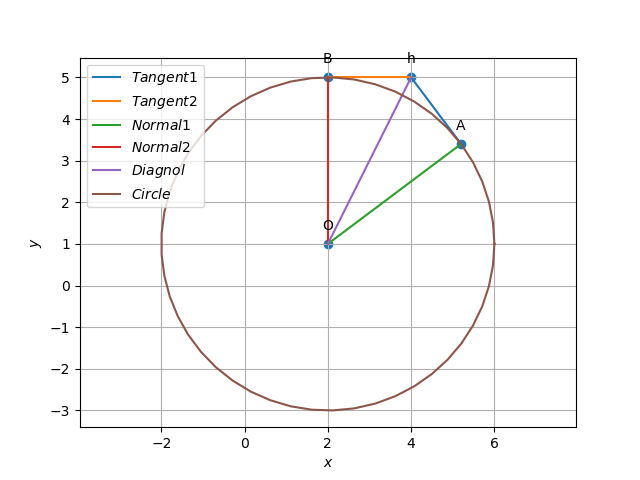
\includegraphics[width=1\columnwidth]{circle.png}
\caption{pair of tangents from point P}
\end{figure}
	\section*{Construction}
\vspace{2mm}
 the input parameters are as follows
{
\setlength\extrarowheight{4pt}
 
 \begin{tabular}{|c|c|c|}
	\hline
	\textbf{Symbol}&\textbf{Value}&\textbf{Description}\\
	\hline
 r&2
	&radius \\
	\hline
 d&rcsc($\theta$)
	&radius of the circle\\
	\hline
l&rcot($\theta$)&tangent(s) of the circle\\
\hline
 \end{tabular}
}
\section*{\large solution}

\subsection*{\large part 1}
Hence from the given equation $x^2+y^2+4x-6y+9sin^2\alpha+13cos^2\alpha=0$\\
\begin{equation}
\vec{O}=(-2,3)\hspace{1em} and \hspace{1em}\vec{r}=\vec{\sqrt{u^T.u-f}}=2\sin\alpha
\end{equation}

hence from Pythagoras theorem sin$\alpha$=OR/OP.Here OR=2sin$\alpha$.\\
\begin{equation}
\sin\alpha=2\sin\alpha/OP.
\end{equation}
\begin{equation}
    \sin^2\alpha=4\sin^2\alpha/OP^2.
\end{equation}
\begin{equation}
\vec{OP^2} sin^2\alpha=4sin^2\alpha
\end{equation}
\begin{equation}
   \vec{OP^2}=4
\end{equation}
\begin{equation}
    \myvec{OP^2}=\vec{\norm{P-O}^2}
\end{equation}
\begin{equation}
\vec{P}=\vec{X},\vec{O}=-\vec{u}
\end{equation}
\begin{equation}
    \vec{\norm{X+u}^2}=4
\end{equation}
\begin{equation}
\vec{(X+u)^T.(X+u)}=4
\end{equation}
\begin{equation}
\vec{\norm{X}^2+\norm{u}^2+2X^Tu}=4
\end{equation}
Hence locus of $\vec{OP}$  upon simplifying is
\begin{equation}
\vec{u}=\myvec{2,-3},\vec{f}=4,\vec{f_1}=\vec{u^T.u-f}
\end{equation}
\begin{equation}
\vec{V}=\vec{I},\vec{u}=-O\vec{u},f_1=9.
\end{equation}
The required locus equation is 
\begin{equation}
\vec{X^T.X+2\vec{u^T}\vec{X}+f_1}=0
\label{eq-5}
\end{equation}
Hence the parameters of the above equation
\begin{equation}
\vec{u}=(2,-3),f_1=9.
\end{equation}
\end{document}
